% Native publication figure; requires tikz and arrows.meta.
% Preserve the adjacent coordinate table as a text equivalent.
\begin{figure}[htbp]
\centering
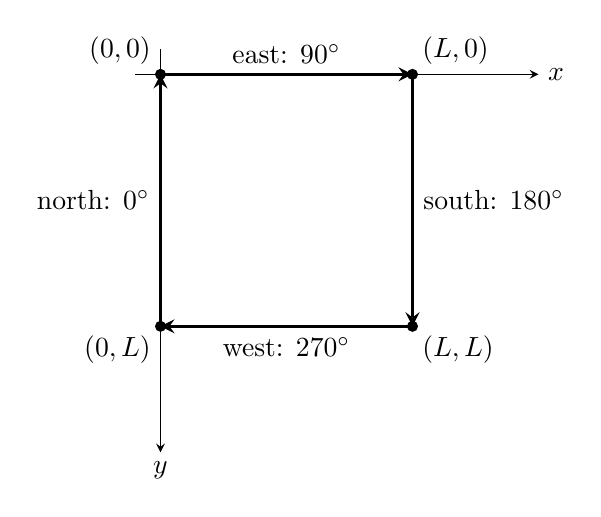
\begin{tikzpicture}[x=0.8cm,y=-0.8cm,>=stealth]
\draw[->] (-0.4,0)--(6,0) node[right] {$x$};
\draw[->] (0,-0.4)--(0,6) node[below] {$y$};
\draw[very thick,->] (0,0)--(4,0) node[midway,above] {east: $90^\circ$};
\draw[very thick,->] (4,0)--(4,4) node[midway,right] {south: $180^\circ$};
\draw[very thick,->] (4,4)--(0,4) node[midway,below] {west: $270^\circ$};
\draw[very thick,->] (0,4)--(0,0) node[midway,left] {north: $0^\circ$};
\fill (0,0) circle (2pt) node[above left] {$(0,0)$};
\fill (4,0) circle (2pt) node[above right] {$(L,0)$};
\fill (4,4) circle (2pt) node[below right] {$(L,L)$};
\fill (0,4) circle (2pt) node[below left] {$(0,L)$};
\end{tikzpicture}
\caption{A clockwise square in screen coordinates. The robot starts at the upper-left corner, and positive $y$ points down. $L$ is the input side length.}
\label{fig:robot-square}
\end{figure}
